\documentclass[border=2mm]{standalone}
\usepackage{pgfplots}
\pgfplotsset{compat=newest}
\begin{document}
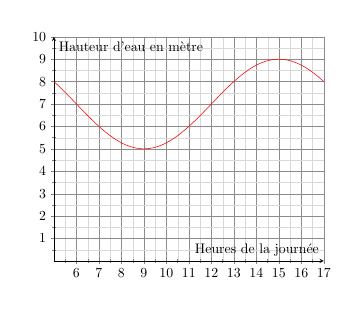
\begin{tikzpicture}[yscale=0.5,xscale=0.5]
  \begin{axis}%
    [grid=both,
     minor tick num=1,
     grid style={line width=.1pt, draw=gray!30},
     major grid style={line width=.2pt,draw=gray!90},
     axis lines=middle,
     xmin=5,xmax=17,ymin=0,ymax=10,
     xtick={5,6,7,8,9,10,11,12,13,14,15,16,17},
     xticklabels={5,6,7,8,9,10,11,12,13,14,15,16,17},
     ytick={0,1,2,3,4,5,6,7,8,9,10},
     yticklabels={0,1,2,3,4,5,6,7,8,9,10},
     xlabel=Heures de la journée,
     ylabel=Hauteur d'eau en mètre
    ]
    \addplot[domain=5:17,samples=50,smooth,red] {2*cos(deg(pi*(x+9)/6)) + 7};
  \end{axis}
\end{tikzpicture}
\end{document}